\section{Engine and Transmission Module}

The engine and transmission module implements the design specified in Sec.\ \ref{sec:engine_transmission_design}. The hardware and software aspects of this module's implementation are discussed in this section.

\subsection{Hardware}

In addition to the base system hardware common to all modules described in Sec.\ \ref{sec:base_system_hardware}, 3 additional hardware components were added. The high-current solenoid drivers specified in the design in Sec. \ref{sec:design_engine_transmission_hardware} were implemented with a single SPI capable octal \emph{low-side solenoid driver}. This driver chip responds to commands over SPI, and switches the low side output pins accordingly. It includes flyback protection circuitry to squash voltage spikes from the inductive load of the solenoid, and can also detect electrical shorts. Additionally, a CMOS buffer chip was added to interface the discrete pins on the ECU (described in Sec.\ \ref{sec:ecu_background_discrete_inputs}), and an SPI capable DAC was added to output the \unit{0-5}{\volt} signal required for setting the traction control slip percentage.

\begin{figure}[H]
\centering
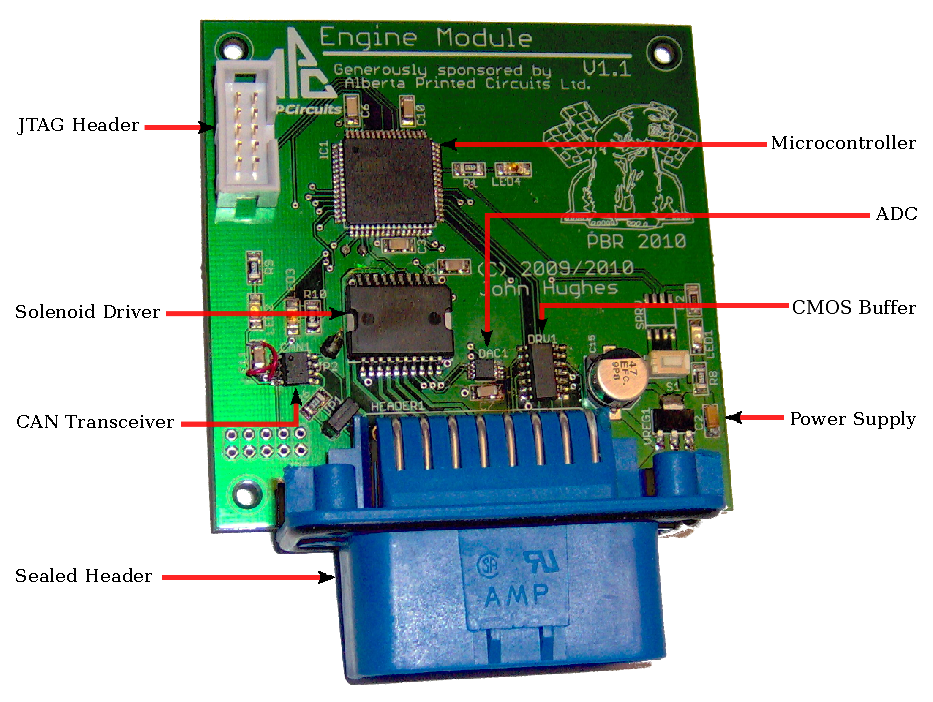
\includegraphics[scale=1]{implementation/figures/engine_transmission_pcb}
\caption{Populated Engine and Transmission module PCB.}
\label{fig:engine_transmission_pcb}
\end{figure}

Figure \ref{fig:engine_system_overview} shows a block-level diagram of the hardware implementation of the engine and transmission module, including the specific components chosen for the imlementation. A list of the components additional to the base system hardware can be found in Table \ref{tab:engine_transmission_module_components}. Descriptions of these components are in the following sections.

\begin{figure}[H]
\centering
\begin{tikzpicture}[auto, node distance=3.5cm, draw=black!70, >=stealth']
  \node [block, name=at90] {AT90CAN};
  \node [block, name=dac, left of=at90] {TLV5623 DAC};
  \node [block, name=driver, right of=at90] {L9822E Solenoid Driver};
  \node [block, name=can, below of=at90, above=0.5cm] {MCP2551 CAN Transceiver};
  \node [block, name=buf, left of=can] {74LVC07 Buffer};

  \node [block, name=ecu, rotate=90, minimum width=8em] at ($(dac.west)!0.5!(buf.west)+(-1.25cm,0)$) {ECU};
  \node [block, name=solenoids, right of=driver, left=-0.75cm] {Solenoids};
  \node [block, name=feedback, below of=solenoids, above=0.75cm, text width=2.2cm, inner sep=0.05cm] {Position Transducers};

  \path (at90.north)+(0.0,+0.4) node (title) {Engine Module};

  \begin{pgfonlayer}{background}
    \path (dac.north west)+(-0.3,0.7) node (a) {};
    \path (can.south -| driver.east)+(+0.3,-0.2) node (b) {};
    \path[module] (a) rectangle (b);
  \end{pgfonlayer}

  \node [bus, name=can1, below of=can, label=below:CAN Bus, above=2.0cm] {CAN Bus};
  \node [bus, name=can2, left of=can1] {};
  \node [bus, name=can3, right of=can1] {};

  \draw [-, line width=3pt] (can) -- (can1);
  \draw [-, line width=3pt] (can1) -- (can2);
  \draw [-, line width=3pt] (can1) -- (can3);

  \draw [->, thick] (driver) -- (solenoids);

  \draw [->, thick] (at90) -- node[above] {SPI} (driver);
  \draw [<->, thick] (at90) -- (can);
  \draw [->, thick] (at90) -- node[above] {SPI} (dac);
  \draw [->, thick] ($(at90.west)+(0,-0.3)$) to[myncbar, arm=0.5cm, angle=180] (buf);
  \draw [<-, thick] ($(at90.east)+(0,-0.3)$) to[myncbar, arm=0.5cm] (feedback);

  \draw [->, thick] (dac.west) to[myncbar, arm=0.2cm, angle=180] ($(ecu.south)+(0,0.5)$);
  \draw [->, thick] (buf.west) to[myncbar, arm=0.2cm, angle=180] ($(ecu.south)+(0,-0.5)$);
% 
% 
%   \draw [-, line width=2pt] (can1) -- (can2);
%   \draw [-, line width=2pt] (can2) -- node[rotate=90, above] {CAN Bus} (can3);
%   \draw [-, line width=2pt] (can3) -- (can4);
% 
%   \node [bus, above of=can1, below=1cm] (tip1) {};
%   \node [bus, below of=can4, above=1cm] (tip2) {};
%   \draw [-, densely dashed, line width=2pt] (can1) -- (tip1);
%   \draw [-, densely dashed, line width=2pt] (can4) -- (tip2);
% 
%   \node [block, right of=can2, right, text width=8em] (engine) {Engine Module};
%   \node [block, right of=can3, right, text width=8em] (ecu) {ECU};
% 
%   \node [block, right of=engine, right, text width=8em] (starter) {Starter System};
%   \node [block, right of=ecu, right, text width=8em] (intake) {Intake System};
%   \node [block, above of=starter, text width=8em] (transmission) {Transmission System};
% 
%   \draw [<->] (engine) -- (ecu);
%   \draw [<->] (engine.south east) -- (intake.north west);
%   \draw [<->] (engine) -- (starter);
%   \draw [<->] (engine.north east) -- (transmission.south west);
% 
%   \draw [<->, line width=2pt] (can2) -- (engine);
%   \draw [<->, line width=2pt] (can3) -- (ecu);
\end{tikzpicture}
\caption{Engine and transmission module hardware overview.}
\label{fig:engine_system_overview}
\end{figure}

\begin{table}
  \caption{Engine and Transmission module components.\label{tab:engine_transmission_module_components}}
  \centering
  \begin{tabular}{|c|c|c|}
    \hline 
    Part & Manufacturer & Part Number\tabularnewline 
    \hline \hline
    Solenoid Driver & ST Microelectronics & L9822E \tabularnewline
    \hline
    Digital to Analogue Converter & Texas Instruments & TLV5623C \tabularnewline
    \hline
    Hex CMOS Buffer & Texas Instruments & 74LVC07A \tabularnewline
    \hline
  \end{tabular}
\end{table}


\subsubsection{High Current Solenoid Driver}

In order to meet the requirement of being able to energize the multiple solenoids specified in the design, an 8-way solenoid driver component from ST Microelectronics was chosen. The LT9822E provides a simple SPI interface for the microcontroller to talk to, and also takes care of possible flyback from the solenoids with built-in clamping diodes.

Using this single component strongly reduces the complexity of the output stage of the circuit, since multiple discrete high-current transistors were not needed.

\subsubsection{Input Buffers}


\subsubsection{Traction Control Analogue Output}

In order to generate a 0-5V analogue signal for the ECU's traction slip ratio input, as was described in Sec. \ref{sec:background_ecu_data_interfaces}, a simple SPI interfaced digital to analogue converter (DAC) from Texas Instruments was introduced. The TLV5623 outputs \unit{0-5}{\volt} analogue signal that varies with the digital input.

The output voltage from the DAC can be determined by the following equation:

\begin{equation}
V_{out}=2\cdot{V_{ref}}\,\frac{Code}{2^{n}}\,\volt
\end{equation}

where $V_{ref}$ is the reference voltage input to the chip, $n=8\,(bits)$, and $Code$ is the digital input value ranging from $0$ to $2^{n-1}$. Since we want to output $\unit{5}{\volt}$ at fullscale input,

\begin{equation}
2\cdot{V_{ref}}\,\frac{2^{7}}{2^{8}}=V_{ref}=\unit{5}{\volt}
\end{equation}.

The DC input resistance $R_{in}$ on the traction cut input pin on the ECU was measured using a series resistor with the input terminal to be $R_{in}\approx\unit{155}{\kilo\ohm}$. The output current of the DAC therefore will be at most $I_{out}=\frac{5v}{155k}\approx\unit{32.26}{\micro\ampere}$.

\subsection{Software}

<Software interface map>


\subsubsection{Transmission Manager}


\subsubsection{Intake Manager}


\subsubsection{Starter Manager}


\subsubsection{Event Scheduler}


\subsubsection{CAN Interface}

<Data flow diagram>


\subsubsection{PWM Generator}

An efficient method was devised to generate 2 synchronized PWM signals from the L9822E driver chip. The $32\, kHz$ external crystal was used as the input to the 8-bit TIM2 timer periferal on the microcontroller. The input to the timer was first scaled by 8 which provided a timebase:
\begin{equation}
TB=\frac{32.768\, kHz}{8}=4.096\, kHz
\end{equation}

The timebase period is then given by:
\begin{equation}
\frac{1}{TB}\approx244\,\mu{S}
\end{equation}

We then define a constant scaling factor for the PWM generator:
\begin{equation}
{PWM\_DUTY\_SCALE}=\frac{T_{PWM}}{TB}\approx205
\end{equation}

By loading the timers compare register with with a value scaled with the constant scaling factor, we can cause the timer to generate an interrupt precisely when a level change in the PWM is required.

When generating 2 waveforms with the same timer periferal, 8 combinations of duty cycles of channels A and B were identified, and can be seen in Figure \ref{fig:pwm_cases}.

Since the waveforms are synchronized, it can be seen that there are only 2 cases where 3 transitions per period are required, corresponding to \ref{fig:pwm_cases_1} and \ref{fig:pwm_cases_2}. This happens when both channels have $0<Duty<100\%$. 2 cases are also apparent when no transitions are required, shown in \ref{fig:pwm_cases_7} and \ref{fig:pwm_cases_8}.

An efficient generating routine was constructed to effect the level transitions and to reset the timer to interrupt at the next transition. For the two cases requiring 3 transitions per period, the timer interrupts 3 times per period. For the two cases where both channels have duty cycle between 0 and 100\%, the routine still interrupts once to allow for a change in duty cycle. For the rest of the cases described, the timer only interrupts twice per PWM period.

\begin{figure}[ht]
  \centering
  \subfigure[Case 1]
  {
    \label{fig:pwm_cases_1}
    \begin{tikztimingtable}
      $PWM_A$		& G 4H 4L \\
      $PWM_B$		& G 2H 6L \\
    \end{tikztimingtable}
  }
  \subfigure[Case 2]
  {
  \label{fig:pwm_cases_2}
  \begin{tikztimingtable}
    $PWM_A$		& G 4H 4L \\
    $PWM_B$		& G 6H 2L \\
  \end{tikztimingtable}
  }
  \subfigure[Case 3]
  {
  \label{fig:pwm_cases_3}
  \begin{tikztimingtable}
    $PWM_A$		& G 4H 4L \\
    $PWM_B$		& 8L \\
  \end{tikztimingtable}
  }
  \subfigure[Case 4]
  {
  \label{fig:pwm_cases_4}
  \begin{tikztimingtable}
    $PWM_A$		& G 4H 4L \\
    $PWM_B$		& G 8H G \\
  \end{tikztimingtable}
  }
  \subfigure[Case 5]
  {
  \label{fig:pwm_cases_5}
  \begin{tikztimingtable}
    $PWM_A$		& G 8H G \\
    $PWM_B$		& G 4H 4L \\
  \end{tikztimingtable}
  }
  \subfigure[Case 6]
  {
  \label{fig:pwm_cases_6}
  \begin{tikztimingtable}
    $PWM_A$		& 8L \\
    $PWM_B$		& G 4H 4L \\
  \end{tikztimingtable}
  }
  \subfigure[Case 7]
  {
  \label{fig:pwm_cases_7}
  \begin{tikztimingtable}
    $PWM_A$		& 8L \\
    $PWM_B$		& 8L \\
  \end{tikztimingtable}
  }
  \subfigure[Case 8]
  {
  \label{fig:pwm_cases_8}
  \begin{tikztimingtable}
    $PWM_A$		& G 8H G \\
    $PWM_B$		& G 8H G \\
  \end{tikztimingtable}
  }
  \caption{PWM Cases (1 period shown).}
  \label{fig:pwm_cases}
\end{figure}

\subsubsection{Main Control Loop}